% Created 2021-03-08 man 19:02
% Intended LaTeX compiler: pdflatex
\documentclass[12pt]{article}

%%%% settings when exporting code %%%% 

\usepackage{listings}
\lstdefinestyle{code-small}{
backgroundcolor=\color{white}, % background color for the code block
basicstyle=\ttfamily\small, % font used to display the code
commentstyle=\color[rgb]{0.5,0,0.5}, % color used to display comments in the code
keywordstyle=\color{black}, % color used to highlight certain words in the code
numberstyle=\ttfamily\tiny\color{gray}, % color used to display the line numbers
rulecolor=\color{black}, % color of the frame
stringstyle=\color[rgb]{0,.5,0},  % color used to display strings in the code
breakatwhitespace=false, % sets if automatic breaks should only happen at whitespace
breaklines=true, % sets automatic line breaking
columns=fullflexible,
frame=single, % adds a frame around the code (non,leftline,topline,bottomline,lines,single,shadowbox)
keepspaces=true, % % keeps spaces in text, useful for keeping indentation of code
literate={~}{$\sim$}{1}, % symbol properly display via latex
numbers=none, % where to put the line-numbers; possible values are (none, left, right)
numbersep=10pt, % how far the line-numbers are from the code
showspaces=false,
showstringspaces=false,
stepnumber=1, % the step between two line-numbers. If it's 1, each line will be numbered
tabsize=1,
xleftmargin=0cm,
emph={anova,apply,class,coef,colnames,colNames,colSums,dim,dcast,for,ggplot,head,if,ifelse,is.na,lapply,list.files,library,logLik,melt,plot,require,rowSums,sapply,setcolorder,setkey,str,summary,tapply},
aboveskip = \medskipamount, % define the space above displayed listings.
belowskip = \medskipamount, % define the space above displayed listings.
lineskip = 0pt} % specifies additional space between lines in listings
\lstset{style=code-small}
%%%% packages %%%%%

\usepackage[utf8]{inputenc}
\usepackage[T1]{fontenc}
\usepackage{lmodern}
\usepackage{textcomp}
\usepackage{color}
\usepackage{graphicx}
\usepackage{grffile}
\usepackage{wrapfig}
\usepackage{rotating}
\usepackage{longtable}
\usepackage{multirow}
\usepackage{multicol}
\usepackage{changes}
\usepackage{pdflscape}
\usepackage{geometry}
\usepackage[normalem]{ulem}
\usepackage{amssymb}
\usepackage{amsmath}
\usepackage{amsfonts}
\usepackage{dsfont}
\usepackage{array}
\usepackage{ifthen}
\usepackage{hyperref}
\usepackage{natbib}
\RequirePackage{setspace} % to modify the space between lines - incompatible with footnote in beamer
\renewcommand{\baselinestretch}{1.1}
\geometry{top=1cm}
\usepackage{titlesec}
\usepackage{etoolbox}
\makeatletter
\patchcmd{\ttlh@hang}{\parindent\z@}{\parindent\z@\leavevmode}{}{}
\patchcmd{\ttlh@hang}{\noindent}{}{}{}
\makeatother
\RequirePackage{colortbl} % arrayrulecolor to mix colors
\definecolor{myorange}{rgb}{1,0.2,0}
\definecolor{mypurple}{rgb}{0.7,0,8}
\definecolor{mycyan}{rgb}{0,0.6,0.6}
\newcommand{\lightblue}{blue!50!white}
\newcommand{\darkblue}{blue!80!black}
\newcommand{\darkgreen}{green!50!black}
\newcommand{\darkred}{red!50!black}
\definecolor{gray}{gray}{0.5}
\hypersetup{
citecolor=[rgb]{0,0.5,0},
urlcolor=[rgb]{0,0,0.5},
linkcolor=[rgb]{0,0,0.5},
}
\newenvironment{comment}{\small \color{gray}\fontfamily{lmtt}\selectfont}{\par}
\newenvironment{activity}{\color{orange}\fontfamily{qzc}\selectfont}{\par}
\RequirePackage{pifont}
\RequirePackage{relsize}
\newcommand{\Cross}{{\raisebox{-0.5ex}%
{\relsize{1.5}\ding{56}}}\hspace{1pt} }
\newcommand{\Valid}{{\raisebox{-0.5ex}%
{\relsize{1.5}\ding{52}}}\hspace{1pt} }
\newcommand{\CrossR}{ \textcolor{red}{\Cross} }
\newcommand{\ValidV}{ \textcolor{green}{\Valid} }
\usepackage{stackengine}
\usepackage{scalerel}
\newcommand\Warning[1][3ex]{%
\renewcommand\stacktype{L}%
\scaleto{\stackon[1.3pt]{\color{red}$\triangle$}{\tiny\bfseries !}}{#1}%
\xspace
}
\newcommand\Rlogo{\textbf{\textsf{R}}\xspace} %
\RequirePackage{fancyvrb}
\DefineVerbatimEnvironment{verbatim}{Verbatim}{fontsize=\small,formatcom = {\color[rgb]{0.5,0,0}}}
\RequirePackage{enumitem} % better than enumerate
\RequirePackage{epstopdf} % to be able to convert .eps to .pdf image files
\RequirePackage{capt-of} %
\RequirePackage{caption} % newlines in graphics
\RequirePackage{tikz-cd} % graph
\RequirePackage{booktabs} % for nice lines in table (e.g. toprule, bottomrule, midrule, cmidrule)
\RequirePackage{amsmath}
\RequirePackage{algorithm}
\RequirePackage[noend]{algpseudocode}
\RequirePackage{dsfont}
\RequirePackage{amsmath,stmaryrd,graphicx}
\RequirePackage{prodint} % product integral symbol (\PRODI)
\usepackage{ifthen}
\usepackage{xifthen}
\usepackage{xargs}
\usepackage{xspace}
\newcommand\defOperator[7]{%
\ifthenelse{\isempty{#2}}{
\ifthenelse{\isempty{#1}}{#7{#3}#4}{#7{#3}#4 \left#5 #1 \right#6}
}{
\ifthenelse{\isempty{#1}}{#7{#3}#4_{#2}}{#7{#3}#4_{#1}\left#5 #2 \right#6}
}
}
\newcommand\defUOperator[5]{%
\ifthenelse{\isempty{#1}}{
#5\left#3 #2 \right#4
}{
\ifthenelse{\isempty{#2}}{\underset{#1}{\operatornamewithlimits{#5}}}{
\underset{#1}{\operatornamewithlimits{#5}}\left#3 #2 \right#4}
}
}
\newcommand{\defBoldVar}[2]{
\ifthenelse{\equal{#2}{T}}{\boldsymbol{#1}}{\mathbf{#1}}
}
\newcommandx\Esp[2][1=,2=]{\defOperator{#1}{#2}{E}{}{\lbrack}{\rbrack}{\mathbb}}
\newcommandx\Prob[2][1=,2=]{\defOperator{#1}{#2}{P}{}{\lbrack}{\rbrack}{\mathbb}}
\newcommandx\Qrob[2][1=,2=]{\defOperator{#1}{#2}{Q}{}{\lbrack}{\rbrack}{\mathbb}}
\newcommandx\Var[2][1=,2=]{\defOperator{#1}{#2}{V}{ar}{\lbrack}{\rbrack}{\mathbb}}
\newcommandx\Cov[2][1=,2=]{\defOperator{#1}{#2}{C}{ov}{\lbrack}{\rbrack}{\mathbb}}
\newcommandx\Binom[2][1=,2=]{\defOperator{#1}{#2}{B}{}{(}{)}{\mathcal}}
\newcommandx\Gaus[2][1=,2=]{\defOperator{#1}{#2}{N}{}{(}{)}{\mathcal}}
\newcommandx\Wishart[2][1=,2=]{\defOperator{#1}{#2}{W}{ishart}{(}{)}{\mathcal}}
\newcommandx\Likelihood[2][1=,2=]{\defOperator{#1}{#2}{L}{}{(}{)}{\mathcal}}
\newcommandx\logLikelihood[2][1=,2=]{\defOperator{#1}{#2}{\ell}{}{(}{)}{}}
\newcommandx\Information[2][1=,2=]{\defOperator{#1}{#2}{I}{}{(}{)}{\mathcal}}
\newcommandx\Score[2][1=,2=]{\defOperator{#1}{#2}{S}{}{(}{)}{\mathcal}}
\newcommandx\Vois[2][1=,2=]{\defOperator{#1}{#2}{V}{}{(}{)}{\mathcal}}
\newcommandx\IF[2][1=,2=]{\defOperator{#1}{#2}{IF}{}{(}{)}{\mathcal}}
\newcommandx\Ind[1][1=]{\defOperator{}{#1}{1}{}{(}{)}{\mathds}}
\newcommandx\Max[2][1=,2=]{\defUOperator{#1}{#2}{(}{)}{min}}
\newcommandx\Min[2][1=,2=]{\defUOperator{#1}{#2}{(}{)}{max}}
\newcommandx\argMax[2][1=,2=]{\defUOperator{#1}{#2}{(}{)}{argmax}}
\newcommandx\argMin[2][1=,2=]{\defUOperator{#1}{#2}{(}{)}{argmin}}
\newcommandx\cvD[2][1=D,2=n \rightarrow \infty]{\xrightarrow[#2]{#1}}
\newcommandx\Hypothesis[2][1=,2=]{
\ifthenelse{\isempty{#1}}{
\mathcal{H}
}{
\ifthenelse{\isempty{#2}}{
\mathcal{H}_{#1}
}{
\mathcal{H}^{(#2)}_{#1}
}
}
}
\newcommandx\dpartial[4][1=,2=,3=,4=\partial]{
\ifthenelse{\isempty{#3}}{
\frac{#4 #1}{#4 #2}
}{
\left.\frac{#4 #1}{#4 #2}\right\rvert_{#3}
}
}
\newcommandx\dTpartial[3][1=,2=,3=]{\dpartial[#1][#2][#3][d]}
\newcommandx\ddpartial[3][1=,2=,3=]{
\ifthenelse{\isempty{#3}}{
\frac{\partial^{2} #1}{\partial #2^2}
}{
\frac{\partial^2 #1}{\partial #2\partial #3}
}
}
\newcommand\Real{\mathbb{R}}
\newcommand\Rational{\mathbb{Q}}
\newcommand\Natural{\mathbb{N}}
\newcommand\trans[1]{{#1}^\intercal}%\newcommand\trans[1]{{\vphantom{#1}}^\top{#1}}
\newcommand{\independent}{\mathrel{\text{\scalebox{1.5}{$\perp\mkern-10mu\perp$}}}}
\newcommand\half{\frac{1}{2}}
\newcommand\normMax[1]{\left|\left|#1\right|\right|_{max}}
\newcommand\normTwo[1]{\left|\left|#1\right|\right|_{2}}
\newcommand\Veta{\boldsymbol{\eta}}
\newcommand\VX{\mathbf{X}}
\newcommand\model{\mathcal{M}}
\author{Brice Ozenne}
\date{\today}
\title{Assessing the effect of an exposure on multiple outcomes (with \Rlogo{} code)}
\hypersetup{
 colorlinks=true,
 pdfauthor={Brice Ozenne},
 pdftitle={Assessing the effect of an exposure on multiple outcomes (with \Rlogo{} code)},
 pdfkeywords={},
 pdfsubject={},
 pdfcreator={Emacs 27.0.50 (Org mode 9.0.4)},
 pdflang={English}
 }
\begin{document}

\maketitle

\section*{Summary}
\label{sec:org9e7a178}
We describe a strategy to assess the effect of an exposure (e.g. a
disease, a genetic factor) on several outcomes (e.g. psychological
outcomes, the binding potential measured in several brain regions)
while accounting for possible risk factors and confounders. This
strategy, called \emph{multiple univariage regressions} strategy, models
the relationship between each outcome and the exposure using a
separate model. Once the models have been correctly fitted, a global
test can be used to test whether there is any effect of the exposure
on the outcomes. After that, multiple tests are performed to test
outcome-specific effects of the exposure where the Dunnett adjustment
is used to control the type 1 error \citep{pipper2012versatile}. An
adjustment is used to improved the control of the type 1 error in
small sample sizes (e.g. n<100). This adjustment has been shown to
beneficial in several settings (using simulation studies) but does not
always perfectly control the type 1 error rate. It is advised to check
that validity of the adjustment when using very small samples or
models with many parameters.

\bigskip

The proposed strategy can be used with any type of outcomes for which
  a can fit a model with asymptotically linear estimators
  (\cite{tsiatis2007semiparametric}, section 3). This includes
  generalized linear model or Cox models. It makes it very flexible
  and the strategy makes only few assumptions on the joint
  distribution. The drawback is that it is not the most efficient
  approach. For instance modelling the joint distribution of the
  outcomes, e.g. using a latent variable model / mixed model in the
  case of normally distributed outcomes, will be a more efficient
  strategy. Another limitation is that with the proposed approach a
  treatment effect specific to each outcome will be estimated, while
  in some context the investigator may want to constrain the treatment
  effect to be the same for some outcomes. Finally, to be feasible the
  strategy requires the number of outcomes to be not too large (<100)
  and smaller than the number of observations (low-dimensional
  setting).

\bigskip

This document we aim at giving a basic understanding of the strategy
  and how to implement it. In particular, we don't claim that the
  proposed strategy is valid or optimal results in every
  application. We start by simulating some data in section
  \ref{sec:simulation}. Section \ref{sec:statistics} is a summary of important
  aspects in applied statistics. Finally section \ref{sec:multipleLM}
  describe the \emph{multiple univariage regressions} strategy.

\clearpage

\section{Simulation of the data}
\label{sec:simulation}
To be able to assess the validity of the proposed strategy, we will
use simulated data containing:
\begin{itemize}
\item a variable identifying each patient: \texttt{Id}
\item 10 outcomes per patient: \texttt{Y1} to \texttt{Y10}.
\item 3 possible exposures per patient: \texttt{age} that is not related to the outcomes, \texttt{BMI}
that has the same effect on all outcomes, and \texttt{MDI} that has a
different effect per outcome.
\end{itemize}
We use the \texttt{lvm} function from the \emph{lava} package to define these variables:
\lstset{language=r,label= ,caption= ,captionpos=b,numbers=none}
\begin{lstlisting}
m.sim <- lava::lvm(Y1 ~ 0*age + 0.25*BMI + 0.1*MDI + 1*eta,
		   Y2[0:2] ~ 0*age + 0.25*BMI + 0.2*MDI + 2*eta,
		   Y3 ~ 0*age + 0.25*BMI + 0.15*MDI + 3*eta,
		   Y4[0:0.5] ~ 0*age + 0.25*BMI + 0.175*MDI + 1*eta,
		   Y5[0:3] ~ 0*age + 0.25*BMI + 0.075*MDI + 2*eta 
		   )
transform(m.sim, Id ~ eta) <- function(x){paste0("Subj",1:NROW(x))}
categorical(m.sim, labels = c("male","female")) <-  ~ Gender
distribution(m.sim, ~age) <-  gaussian.lvm(mean = 35, sd = 5)
distribution(m.sim, ~BMI) <-  gaussian.lvm(mean = 22, sd = 3)
distribution(m.sim, ~MDI) <-  gaussian.lvm(mean = 20, sd = 5)
latent(m.sim) <- ~eta
\end{lstlisting}

From the code above we can see that the variance of the outcomes
 differs between outcomes and that the correlation between pairs of
 outcomes is also variable. We now simulate data using \texttt{lava::sim}:
\lstset{language=r,label= ,caption= ,captionpos=b,numbers=none}
\begin{lstlisting}
set.seed(10)
dfW <- lava::sim(m.sim, n = 50, latent = FALSE)
\end{lstlisting}

We round the values to 2 digits:
\lstset{language=r,label= ,caption= ,captionpos=b,numbers=none}
\begin{lstlisting}
digit.cols <- c("age","BMI","MDI",paste0("Y",1:5))
dfW[,digit.cols] <- round(dfW[,digit.cols],2)
\end{lstlisting}

and re-order its columns:
\lstset{language=r,label= ,caption= ,captionpos=b,numbers=none}
\begin{lstlisting}
dfW <- dfW[,c("Id","Gender",digit.cols)]
\end{lstlisting}

\clearpage

We can now display first lines of the dataset:
\lstset{language=r,label= ,caption= ,captionpos=b,numbers=none}
\begin{lstlisting}
head(dfW)
\end{lstlisting}
\begin{verbatim}
     Id Gender   age   BMI   MDI   Y1    Y2    Y3    Y4   Y5
1 Subj1 female 30.57 21.76 25.82 7.64  8.73  7.72 10.42 8.44
2 Subj2 female 41.36 25.55 12.38 7.11  8.79  6.99  8.45 8.26
3 Subj3   male 26.97 28.56  7.41 7.88  9.89 13.51 10.79 7.90
4 Subj4 female 40.61 23.22 16.46 8.99 14.38 13.82 11.44 9.75
5 Subj5 female 45.79 19.78 18.56 7.60  8.77  8.38  7.94 6.17
6 Subj6 female 37.14 16.13 17.82 6.99  9.97  6.74  8.29 8.78
\end{verbatim}

\clearpage

\section{Statistics: definitions and notations}
\label{sec:statistics}
\subsection{Variables}
\label{sec:org97c2cc5}

We can differentiate several types of random variables: outcomes,
exposure, risk factors, confounders, and mediators. To explicit the
difference between these types of variables we consider a set of
random variables \((Y,E,X_1,X_2,M)\) whose relationships are
displayed on \autoref{fig:pathDiagram}:
\begin{itemize}
\item \textbf{outcome} (\(Y\)): random variables that are observed with noise. It
can be for instance the 5HT-4 binding in a specific brain
region. When considering several outcomes we will denote in bold
variable that stands for a vector of random variables:
\(\mathbf{Y}=(Y_1,Y_2,\ldots,Y_m)\). This happens for instance when
studying the binding in several brain regions. In such a case we
expect the outcomes to be correlated.
\item \textbf{exposure} (\(E\)): a variable that may affect the outcome or be
associated with the outcome \emph{and} we are interested in studying this
effect/association. It can for instance be a genetic factor that is
hypothesized to increase the 5HT-4 binding, or a disease like
depression that is associated with a change in binding (we don't
know whether one causes the other or whether they have a common
cause, e.g. a genetic variant).
\item \textbf{risk factor/confounder} (\(X_1,X_2\)): a variable that
may affect the outcome or be associated with the outcomes \emph{but} we
are \emph{not} interested in studying their effect/association. Risk
factors (denoted by \(X_1\)) are only associated with the outcomes
and confounders that are both associated with the outcome and the
exposure. We usually need to account for confounders the statistical
model in order to obtain unbiased estimates while accounting for
risk factors only enables to obtain more precise estimates (at least
in linear models).
\item \textbf{mediator} (\(M\)): a variable that modulate the effect of the
exposure, i.e. stands on the causal pathway between the exposure and
the outcome. For instance, the permeability of the blood-brain
barrier may modulate the response to drugs and can act as a
mediator. It is important to keep in mind that when we are
interested in the (total) effect of \(E\) on \(Y\), we should \emph{not}
adjust the analysis on \(M\)\footnote{This may not be true in specific types of confounding but we
will ignore that.}. Doing so we would remove the effect of
\(E\) mediated by \(M\) and therefore bias the estimate of the total
effect (we would only get the direct effect).
\end{itemize}

In the following we will assume that we do not measure any mediator
variable and therefore ignore this type of variable. Also we will call
\textbf{covariates} the variables \(E,X_1,X_2\).

\begin{figure}[htbp]
\centering
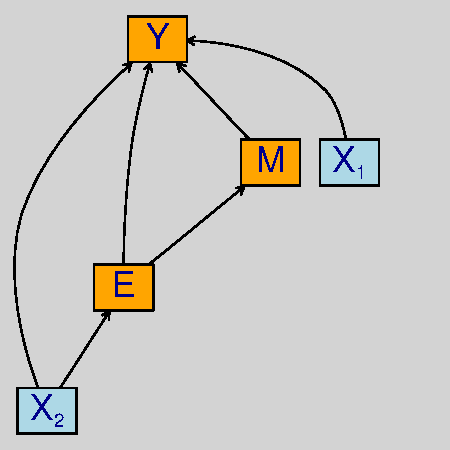
\includegraphics[width=0.7\textwidth]{./figures/pathDiagram.pdf}
\caption{\label{fig:pathDiagram}
Path diagram relating the variables Y, E, M, \(X_1\) and \(X_2\)}
\end{figure}

\clearpage 

\subsection{Assumptions}
\label{sec:orgebb01ae}

We can distinguish two types of assumptions:
\begin{itemize}
\item \textbf{causal assumptions}: saying which variables are related and in
which direction. This can be done by drawing a path diagram similar
to \autoref{fig:pathDiagram}. In simple univariate models it may seems
unnecessary to draw the path diagram since the system of variables is
very simple to visualize. In multivariate model, it is often very
useful to draw it. Some of these assumptions are untestable,
e.g. often we cannot decide whether it is \(E\) that impacts \(Y\)
or whether it is \(Y\) that impacts \(E\) just based on the data.

\item \textbf{modeling assumptions}: specifying the type of relationship between
variables (e.g. linear) and the marginal or joint distribution
(e.g. Gaussian). Often these assumptions can be tested and relaxed
using a more flexible model. While appealing, there are some
drawbacks with using a very flexible model: more data are needed to
get precise estimates and the interpretation of the results is more
complex.
\end{itemize}

\subsection{Statistical model}
\label{sec:org286bccc}
A statistical model \(\model\) is set of possible probability
distributions. For instance when we fit a Gaussian linear model for
\(Y_1\) with just an intercept \(\model=\left\{\Gaus[\mu,\sigma^2];\mu
\in \Real, \; \sigma^2 \in \Real^+ \right\}\): \(\model\) is the set
containing all possible univariate normal distributions.

\subsection{Model parameters}
\label{sec:org93a7194}

The model parameters are the (non random) variables that enable the
statistical model to "adapt" to different settings. They will be
denoted \(\Theta\). They are the one that are estimated when we fit
the statistical model using the data or that we specify when we
simulate data. In the previous example, we could simulate data
corresponding to a Gaussian linear model using the \texttt{rnorm} function in
R:
\lstset{language=r,label= ,caption= ,captionpos=b,numbers=none}
\begin{lstlisting}
rnorm
\end{lstlisting}

\begin{verbatim}
function (n, mean = 0, sd = 1) 
.Call(C_rnorm, n, mean, sd)
<bytecode: 0x88d8050>
<environment: namespace:stats>
\end{verbatim}

We would need to specify:
\begin{itemize}
\item \(n\) the sample size
\item \(\Theta=(\mu,\sigma^2)\) the model parameters, here \(\mu\) corresponds to \texttt{mean} and \(\sigma\) to \texttt{sd}.
\end{itemize}

\bigskip

The true model parameters are the model parameters that have generated
the observed data. They will be denoted \(\Theta_0\). For instance if
in reality the binding potential is normally distributed with mean 5
and variance \(2^2=4\), then
\(\Theta_0=(\mu_0,\sigma_0^2)=(5,4)\). Then doing our experiment we
observed data such as:
\lstset{language=r,label= ,caption= ,captionpos=b,numbers=none}
\begin{lstlisting}
set.seed(10)
Y_1.XP1 <- rnorm(10, mean = 5, sd = 2)
Y_1.XP1
\end{lstlisting}

\begin{verbatim}
[1] 5.037492 4.631495 2.257339 3.801665 5.589090 5.779589 2.583848 4.272648 1.746655 4.487043
\end{verbatim}

If we were to re-do the experiment we would observe new data but \(\Theta_0\) would not change:
\lstset{language=r,label= ,caption= ,captionpos=b,numbers=none}
\begin{lstlisting}
Y_1.XP2 <- rnorm(10, mean = 5, sd = 2)
Y_1.XP2
\end{lstlisting}

\begin{verbatim}
[1] 7.203559 6.511563 4.523533 6.974889 6.482780 5.178695 3.090112 4.609699 6.851043 5.965957
\end{verbatim}

The estimated parameters are the parameters that we estimate when we
fit the statistical model. They will be denoted \(\hat{\Theta}\). We
usually try to find parameters whose value maximize the chance of
simulating the observed data under the estimated model (maximum
likelihood estimation, MLE). For instance in the first experiment all
values are positive so we would not estimate a negative mean value. In
our example, \(\hat{\mu}\) the MLE of \(\mu\) reduces to the empirical
average and \(\hat{\sigma}^2\) the MLE of \(\sigma^2\) to the
empirical variance:
\lstset{language=r,label= ,caption= ,captionpos=b,numbers=none}
\begin{lstlisting}
Theta_hat.XP1 <- c(mu_hat = mean(Y_1.XP1),
		   sigma2_hat = var(Y_1.XP1))
Theta_hat.XP1
\end{lstlisting}

\begin{verbatim}
  mu_hat sigma2_hat 
4.018686   1.959404
\end{verbatim}

Clearly the estimated coefficients vary across experiments:
\lstset{language=r,label= ,caption= ,captionpos=b,numbers=none}
\begin{lstlisting}
Theta_hat.XP2 <- c(mu_hat = mean(Y_1.XP2),
		   sigma2_hat = var(Y_1.XP2))
Theta_hat.XP2
\end{lstlisting}

\begin{verbatim}
  mu_hat sigma2_hat 
5.739183   1.799311
\end{verbatim}

\subsection{Parameter of interest}
\label{sec:orgc426920}

The statistical model may contain many parameters, most of them are
often not of interest but are needed to obtain valid estimates
(e.g. account for confounders). In most settings, the parameter of
interest is one (or several) model parameter(s) - or simple
transformation of them. For instance if we are interested in the
average binding potential in the population our parameter of interest
is \(\mu\).

\bigskip

Often, the aim of a study is to obtain the best estimate of the
parameter of interest \(\mu\). Best means:
\begin{itemize}
\item \textbf{unbiased}: if we were able to replicate the study many times,
i.e. get several estimates \(\hat{\mu}_1,\hat{\mu}_2,\ldots,\hat{\mu}_K\), the
average estimate \(<\hat{\mu}>=\frac{\hat{\mu}_1+\hat{\mu}_2+\ldots+\hat{\mu}_K}{K}\) would coincide with the true one \(\mu_0\).
\item \textbf{minimal variance}: if we were able to replicate the study many
times, the variance of the estimates
\(\frac{(\hat{\mu}_1-<\hat{\mu}>)^2+\ldots+(\hat{\mu}_K-<\hat{\mu}>)^2}{K-1}\)
should be as low as possible.
\end{itemize}

There will often be a trade-off between these two objectives. A very
flexible method is more likely to give an unbiased estimate
(e.g. being able to model non-linear relationship) at the price of
greater uncertainty about the estimates. Often we favor unbiasedness
over minimal variance. Indeed, if several studies are published with
the same parameter of interest, one can pool the results to obtain an
estimate with lower variance. Note that we have no guarantee that it
will reduce the bias.

\subsection{Contrast matrix}
\label{sec:org652af09}

Consider a linear model:
\lstset{language=r,label= ,caption= ,captionpos=b,numbers=none}
\begin{lstlisting}
e.lm <- lm(Y1 ~ Gender + age + MDI, data = dfW)
e.lm
\end{lstlisting}

\begin{verbatim}

Call:
lm(formula = Y1 ~ Gender + age + MDI, data = dfW)

Coefficients:
 (Intercept)  Genderfemale           age           MDI  
     4.77626      -0.02049      -0.02030       0.16403
\end{verbatim}
Denote for the \(i-th\) patient its outcome value by \(Y_i\) (can be
any real number), its gender value by \(Gender_i\) (can be "Male" or
"Female"), its age value by \(age_i\) (can be 60, 35, or 26), and its
BMI value by \(BMI_i\). Mathematically, this linear model can be
written:
\begin{align*}
Y_i =& \alpha + \beta_{Gender} * \Ind[Gender_i="Female"] + \beta_{Age} * Age_i + \beta_{MDI} * MDI_i + \varepsilon_i
\end{align*}
When dealing with many parameters it is convenient to define the null
hypothesis via a contrast matrix. An example of null hypothesis is:
\begin{align*}
(\Hypothesis[0]) \; \beta_{MDI,0} = 0
\end{align*}
If we consider \(\Theta=(\alpha,\beta_{Gender},\beta_{age},\beta_{MDI})\),
this null hypothesis can be equivalently written:

\begin{align*}
c=[0 \; 0 \; 0 \; 1]
\end{align*}
such that: 
\begin{align*}
(\Hypothesis[0]) \; c \trans{\Theta}_{0} = 0
\end{align*}
Indeed
\begin{align*}
c \trans{\Theta}_{0} = 0 * \alpha_0 + 0 * \beta_{Gender,0} + 0 * \beta_{age,0} + 1 * \beta_{MDI,0} = \beta_{MDI,0}
\end{align*}

An example where the contrast matrix is useful is
\begin{itemize}
\item when one wish to test linear combination of parameters,
e.g. consider the null hypothesis where the added risk when being a
female instead of a male is the same as being 5 years older:
\end{itemize}
\begin{align*}
(\Hypothesis[0]) \; 5 \beta_{age,0} = \beta_{Gender,0}
\end{align*}
Here the contrast matrix would be:
\begin{align*}
c=[0 \; 5 \; -1 \; 0]
\end{align*}
\begin{itemize}
\item when one wish to test several hypotheses simultaneously,
e.g. consider the null hypothesis:
\end{itemize}
\begin{align*}
(\Hypothesis[0]) \; \beta_{age,0} = 0 \text{ or } \beta_{MDI,0} = 0 \\
\end{align*}
Here the contrast matrix would be:
\begin{align*}
C = \begin{bmatrix}
0 & 0 & 1 & 0 \\
0 & 0 & 0 & 1 \\
\end{bmatrix}
\end{align*}

\clearpage

In \Rlogo{}, the method \texttt{createContrast} from the \emph{lavaSearch2}
package helps to define the contrast matrix:
\lstset{language=r,label= ,caption= ,captionpos=b,numbers=none}
\begin{lstlisting}
library(lavaSearch2)
Clin <- createContrast(e.lm, par = c("5*age - Genderfemale = 0"),
		       add.variance = FALSE, rowname.rhs = FALSE)
Clin$contrast
\end{lstlisting}

\begin{verbatim}
                     (Intercept) Genderfemale age MDI
Genderfemale - 5*age           0            1  -5   0
\end{verbatim}

\lstset{language=r,label= ,caption= ,captionpos=b,numbers=none}
\begin{lstlisting}
Csim <- createContrast(e.lm, par = c("age = 0","MDI = 0"),
		       add.variance = FALSE, rowname.rhs = FALSE)
Csim$contrast
\end{lstlisting}

\begin{verbatim}
    (Intercept) Genderfemale age MDI
age           0            0   1   0
MDI           0            0   0   1
\end{verbatim}

Then the contrast matrix can be send to the function \texttt{glht} from the \emph{multcomp} package to obtain p-values and
confidence intervals:
\lstset{language=r,label= ,caption= ,captionpos=b,numbers=none}
\begin{lstlisting}
library(multcomp)
elin.glht <- glht(e.lm, linfct = Clin$contrast)
summary(elin.glht)
\end{lstlisting}

\begin{verbatim}

	 Simultaneous Tests for General Linear Hypotheses

Fit: lm(formula = Y1 ~ Gender + age + MDI, data = dfW)

Linear Hypotheses:
                          Estimate Std. Error t value Pr(>|t|)
Genderfemale - 5*age == 0   0.0810     0.5364   0.151    0.881
(Adjusted p values reported -- single-step method)
\end{verbatim}

\clearpage

\lstset{language=r,label= ,caption= ,captionpos=b,numbers=none}
\begin{lstlisting}
esim.glht <- glht(e.lm, linfct = Csim$contrast)
summary(esim.glht)
\end{lstlisting}

\begin{verbatim}
	 Simultaneous Tests for General Linear Hypotheses

Fit: lm(formula = Y1 ~ Gender + age + MDI, data = dfW)

Linear Hypotheses:
         Estimate Std. Error t value Pr(>|t|)    
age == 0 -0.02030    0.04250  -0.478  0.86315    
MDI == 0  0.16403    0.04051   4.049  0.00039 ***
---
Signif. codes:  0 ‘***’ 0.001 ‘**’ 0.01 ‘*’ 0.05 ‘.’ 0.1 ‘ ’ 1
(Adjusted p values reported -- single-step method)
\end{verbatim}

\clearpage


\section{Multivariate analysis using multiple univariate linear regressions}
\label{sec:multipleLM}
We want to simultaneously test the effect of MDI on five outcomes. To
achieve it, we fit separately for each outcome a univariate linear
regression. Mathematically the model can be written:
\begin{align*}
\begin{bmatrix} 
Y_1  &= \alpha_{Y_{1}} + \beta_{Y_1,age} age + \beta_{Y_1,BMI} BMI + \beta_{Y_1,MDI} MDI + \varepsilon_{Y_1} \\
Y_2  &= \alpha_{Y_{2}} + \beta_{Y_2,age} age + \beta_{Y_2,BMI} BMI + \beta_{Y_2,MDI} MDI + \varepsilon_{Y_2} \\
Y_3  &= \alpha_{Y_{3}} + \beta_{Y_3,age} age + \beta_{Y_3,BMI} BMI + \beta_{Y_3,MDI} MDI + \varepsilon_{Y_3} \\
Y_4  &= \alpha_{Y_{4}} + \beta_{Y_4,age} age + \beta_{Y_4,BMI} BMI + \beta_{Y_4,MDI} MDI + \varepsilon_{Y_4} \\
Y_5  &= \alpha_{Y_{5}} + \beta_{Y_5,age} age + \beta_{Y_5,BMI} BMI + \beta_{Y_5,MDI} MDI + \varepsilon_{Y_5} 
\end{bmatrix} 
\end{align*}
where
\(\varepsilon_{1},\varepsilon_{2},\varepsilon_{3},\varepsilon_{4},\varepsilon_{5}\)
are the residual errors. The residuals are assumed to have zero mean
and finite variance, respectively,
\(\sigma^2_{1},\sigma^2_{2},\sigma^2_{3},\sigma^2_{4},\sigma^2_{5}\). Here
we make no assumption on the correlation structure between the
residuals.

\subsection{Fitting multiple linear regression in \Rlogo{}}
\label{sec:org75c5336}

We can estimate all the 5 models and store them into a list:
\lstset{language=r,label= ,caption= ,captionpos=b,numbers=none}
\begin{lstlisting}
ls.lm <- list(Y1 = lm(Y1 ~ age + BMI + MDI, data = dfW),
	      Y2 = lm(Y2 ~ age + BMI + MDI, data = dfW),
	      Y3 = lm(Y3 ~ age + BMI + MDI, data = dfW),
	      Y4 = lm(Y4 ~ age + BMI + MDI, data = dfW),
	      Y5 = lm(Y5 ~ age + BMI + MDI, data = dfW)
	      )
\end{lstlisting}

\subsection{Interpretation of the regression coefficients}
\label{sec:org9196ff8}

Same as in the univariate case (see
\url{https://bozenne.github.io/doc/2020-09-17-linearModel/post-linearModel.pdf}).

\subsection{Diagnostics tools for univariate linear regression in \Rlogo{}}
\label{sec:orgcb16e12}

Same as in the univariate case (see
\url{https://bozenne.github.io/doc/2020-09-17-linearModel/post-linearModel.pdf}). Model
checking needs to be done for each outcome.

\clearpage

\subsection{Hypothesis testing}
\label{sec:orgfe3c9b6}

We now want to test:
\begin{align*}
(\Hypothesis[0]) \; \beta_{Y_1, MDI, 0} = 0
 \text{ and } \beta_{Y_2, MDI, 0} = 0
 \text{ and } \beta_{Y_3, MDI, 0} = 0
 \text{ and } \beta_{Y_4, MDI, 0} = 0
 \text{ and } \beta_{Y_5, MDI, 0} = 0
\end{align*}

The p-values returned by \texttt{summary} are no more valid since we are
performing multiple tests (here 5 tests). A basic solution would be to
collect the p-values:
\lstset{language=r,label= ,caption= ,captionpos=b,numbers=none}
\begin{lstlisting}
vec.p.value <- unlist(lapply(ls.lm, function(x){
    summary(x)$coef["MDI","Pr(>|t|)"]
}))
\end{lstlisting}

and adjust them for multiple comparisons using Bonferroni:
\lstset{language=r,label= ,caption= ,captionpos=b,numbers=none}
\begin{lstlisting}
p.adjust(vec.p.value, method = "bonferroni")
\end{lstlisting}

\begin{verbatim}
          Y1           Y2           Y3           Y4           Y5 
3.299432e-04 4.218369e-02 3.552579e-01 2.276690e-07 8.565878e-01
\end{verbatim}

While easy to use this approach tends to be too conservative
(i.e. give to large p-values) when the test statistics are
correlated. This is usually the case when the outcomes are
correlated. We will therefore use a more efficient correction called
the Dunnett approach. First we need to define the null hypothesis
that we want to test via a contrast matrix. For simple null hypotheses
like the one we are considering in this example, we can use the
function \texttt{createContrast} that will create the matrix for us:
\lstset{language=r,label= ,caption= ,captionpos=b,numbers=none}
\begin{lstlisting}
resC <- createContrast(ls.lm, var.test = "MDI", add.variance = TRUE)
\end{lstlisting}

This function defines for each model the appropriate contrast matrix:
\lstset{language=r,label= ,caption= ,captionpos=b,numbers=none}
\begin{lstlisting}
resC$mlf
\end{lstlisting}
\begin{verbatim}
$Y1
    (Intercept) age BMI MDI sigma2
MDI           0   0   0   1      0

$Y2
    (Intercept) age BMI MDI sigma2
MDI           0   0   0   1      0

$Y3
    (Intercept) age BMI MDI sigma2
MDI           0   0   0   1      0

$Y4
    (Intercept) age BMI MDI sigma2
MDI           0   0   0   1      0

$Y5
    (Intercept) age BMI MDI sigma2
MDI           0   0   0   1      0

attr(,"class")
[1] "mlf"
\end{verbatim}

and right hand side of the null hypothesis:
\lstset{language=r,label= ,caption= ,captionpos=b,numbers=none}
\begin{lstlisting}
resC$null
\end{lstlisting}

\begin{verbatim}
Y1: MDI Y2: MDI Y3: MDI Y4: MDI Y5: MDI 
      0       0       0       0       0
\end{verbatim}

We will now call \texttt{glht2} to perform the adjustment for multiple
comparisons but first we need to convert the list into a \texttt{mmm} object:
\lstset{language=r,label= ,caption= ,captionpos=b,numbers=none}
\begin{lstlisting}
class(ls.lm) <- "mmm"
e.glht_lm <- glht2(ls.lm, linfct = resC$contrast, rhs = resC$null)
e.glht_lm
\end{lstlisting}

\begin{verbatim}
	 General Linear Hypotheses

Linear Hypotheses:
             Estimate
Y1: MDI == 0  0.15104
Y2: MDI == 0  0.16770
Y3: MDI == 0  0.14907
Y4: MDI == 0  0.19860
Y5: MDI == 0  0.09806
\end{verbatim}

We can now correct for multiple comparisons using the (single-step)
Dunnett approach:
\lstset{language=r,label= ,caption= ,captionpos=b,numbers=none}
\begin{lstlisting}
summary(e.glht_lm, test = adjusted("single-step"))
\end{lstlisting}

\begin{verbatim}
	 Simultaneous Tests for General Linear Hypotheses

Linear Hypotheses:
             Estimate Std. Error t value Pr(>|t|)    
Y1: MDI == 0  0.15104    0.03441   4.389   <0.001 ***
Y2: MDI == 0  0.16770    0.06093   2.752   0.0286 *  
Y3: MDI == 0  0.14907    0.08067   1.848   0.1996    
Y4: MDI == 0  0.19860    0.03039   6.535   <0.001 ***
Y5: MDI == 0  0.09806    0.07057   1.390   0.4208    
---
Signif. codes:  0 '***' 0.001 '**' 0.01 '*' 0.05 '.' 0.1 ' ' 1
(Adjusted p values reported -- single-step method)
\end{verbatim}

Note that the p-value for the global test equals to the smallest
 p-value. This means that we reject the global null hypothesis
 whenever we reject the null hypothesis for any of the outcome (after
 adjustment for multiple comparisons!).


For comparison one can change the argument in \texttt{adjust} to apply the
Bonferroni adjustment:
\lstset{language=r,label= ,caption= ,captionpos=b,numbers=none}
\begin{lstlisting}
summary(e.glht_lm, test = adjusted("bonferroni"))
\end{lstlisting}

\begin{verbatim}
	 Simultaneous Tests for General Linear Hypotheses

Linear Hypotheses:
             Estimate Std. Error t value Pr(>|t|)    
Y1: MDI == 0  0.15104    0.03441   4.389  0.00033 ***
Y2: MDI == 0  0.16770    0.06093   2.752  0.04218 *  
Y3: MDI == 0  0.14907    0.08067   1.848  0.35526    
Y4: MDI == 0  0.19860    0.03039   6.535 2.28e-07 ***
Y5: MDI == 0  0.09806    0.07057   1.390  0.85659    
---
Signif. codes:  0 '***' 0.001 '**' 0.01 '*' 0.05 '.' 0.1 ' ' 1
(Adjusted p values reported -- bonferroni method)
\end{verbatim}

Finally, confidence intervals can be obtained using the \texttt{confint}
function:
\lstset{language=r,label= ,caption= ,captionpos=b,numbers=none}
\begin{lstlisting}
confint(e.glht_lm)
\end{lstlisting}

\begin{verbatim}
	 Simultaneous Confidence Intervals

Fit: NULL

Quantile = 2.5215
95% family-wise confidence level
 

Linear Hypotheses:
             Estimate lwr      upr     
Y1: MDI == 0  0.15104  0.06427  0.23782
Y2: MDI == 0  0.16770  0.01407  0.32133
Y3: MDI == 0  0.14907 -0.05434  0.35248
Y4: MDI == 0  0.19860  0.12197  0.27524
Y5: MDI == 0  0.09806 -0.07987  0.27599
\end{verbatim}
Note that by default the \texttt{confint} function output confidence
intervals using the (single-step) Dunnett approach.


\clearpage

\section{References}
\label{sec:org17b2da9}

\begingroup
\renewcommand{\section}[2]{}
\bibliographystyle{apalike}
\bibliography{bibliography} 
\endgroup
\end{document}